\section{Grundlagen}

\subsection{Was sind Captchas?}
Die Bezeichnung Captcha steht für "Completely Automated Public Turing test to tell Computers and Humans Apart". Mit Hilfe von Captchas soll ein Menschen von einem Computer unterschieden werden können. Das ist notwendig, um bspw. bei einem Login in ein Softwaresystem den Menschen von einem Computer zu unterscheiden. Der Computer könnte  beliebig oft Passwörter aufprobieren bis es das korrekte Passwort gefunden hat. Wenn jedoch ab dem dritten Versuch eine Validierung des Menschen in Form eines Captchas abgefragt wird, wird dieses Vorgehen deutlich erschwert. Das Captcha Prinzip ist eine Aufgabe (Challenge) und eine richtige Antwort (Response). Die Aufgabe sollte für einen Menschen möglichst sehr einfach lösbar aber für einen Computer sehr schwer sein. Die Aufgabe besteht sehr oft in Form eines Bildes. Auf diesem Bild kann bspw. eine schwer lesbare Zeichenfolge von Buchstaben und Ziffern sein, aber auch ein Objekt, wie bspw. ein Hund. Der Mensch erkennt einen Hund auf einem Bild sofort, jedoch ist die softwareseitige Erkennung  schwer implementierbar. Ein Mensch erkennt einen Hund auch, wenn er die Hunderasse vorher noch nie gesehen hat, weil er in seinem neuronalen Netz im Gehirn lernt, kombiniert und erkennt. Viele Captchas sind Zeichenfolgen, so dass der Mensch die auf dem Bild zu sehende Zeichenfolge in ein Textfeld eingeben muss. Die Zeichenfolge kann dabei etwas gedreht oder gedehnt sein, damit diese nicht einfach durch eine Texterkennungssoftware gelesen werden kann. Captchas werden auch HIP (Human Interaction Proof) genannt.

\begin{figure}[htbp]
  \centering
  \fbox{
    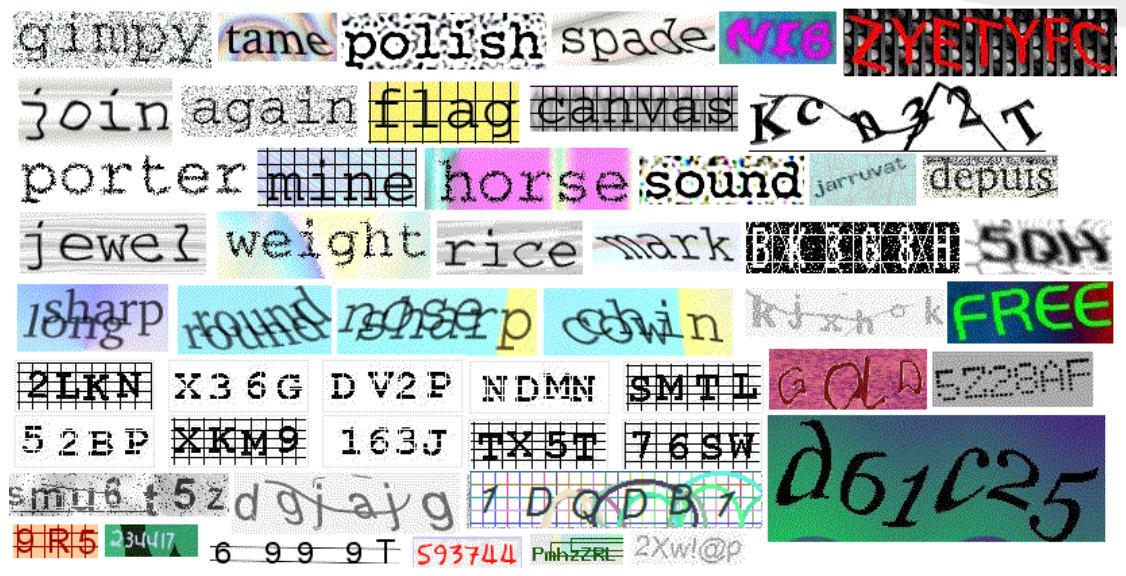
\includegraphics[scale=0.5]{res/captchas.png}
  }
  \caption{Verschiedene Zeichenfolgen Captchas aus der Praxis.}
  \label{Captchas}
\end{figure}

\begin{figure}[htbp]
  \centering
  \fbox{
    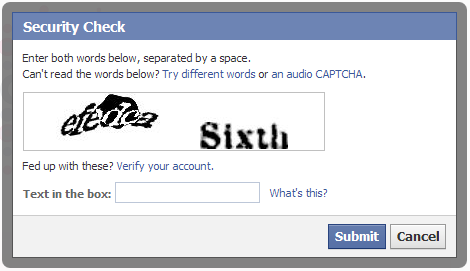
\includegraphics[scale=0.5]{res/catpcha-example.png}
  }
  \caption{Captcha Anwendung bei Facebook.}
  \label{Captchas}
\end{figure}

\newpage

\subsection{Motivation}
Ziel dieses Softcomputing Projekts ist es reale Captchas mit Hilfe von neuronalen Netzen zu dekodieren. Um die Entwicklung zu vereinfachen wurde auf MATLAB gesetzt, da darin bereits Funktionen zur Bildverarbeitung und neuronalen Netzen integriert sind. Dabei wird die Verwendung von neuronalen Netzen studiert und angewandt. Die verwendeten Captchas sind Zeichenfolgen von Buchstaben und Grafiken, die leicht gedreht und mit Mustern im Hintergrund schwerer lesbar gemacht wurden. Es soll gezeigt werden, dass mit einer größeren Menge Captchas das neuronale Netz aufgebaut bzw. trainiert werden kann, um anschließend ähnliche Captchas zu dekodieren. Damit kann die Unterscheidung eines Menschen von einem Computer gebrochen werden, um bspw. Softwaresysteme angreifbar zu machen. 

\subsection{Captcha Generator}
Für den Aufbau des neuronalen Netzes werden viele Captchas inklusive der Lösung benötigt. Um an diese Menge von Captchas zu kommen wurde ein eigener Captcha Generator entwickelt. Der Generator wurde als eine .NET Applikation in C\# realisiert. Der Captcha Generator hat einige Konfigurationsmöglichkeiten: Ausgabeverzeichnis, Anzahl der Zeichen auf einem Bild, Anzahl der Captchas und der Neigungswinkel der einzelnen Zeichen in Grad. Der Generator erzeugt die Captachs im PNG-Bildformat und setzt als Dateinamen die Lösung der Zeichenfolge. Die Captchas können auf diese Art und Weise genutzt werden, um das neuronale Netz aufzubauen und die Erkennung mit dem Dateinamen des Bildes zu validieren.

\begin{figure}[htbp]
  \centering
  \fbox{
    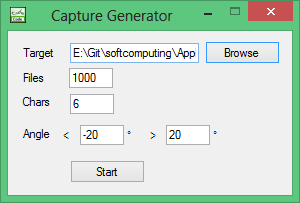
\includegraphics{res/captcha-generator.png}
  }
  \caption{Benutzeroberfläche des Captcha Generators.}
  \label{Captchas}
\end{figure}

\begin{figure}[htbp]
  \centering
  \fbox{
    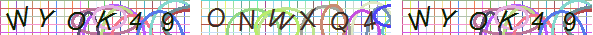
\includegraphics{res/generator-captchas.png}
  }
  \caption{Drei mit dem Generator erzeugte Captchas.}
  \label{Captchas}
\end{figure}
